\chapter{The effect of haptic feedback in the balance task of bicycling}\label{chapter 5}

%\textcolor{black}{->Corresponding article: G. Dialynas, R. Happee, A. L. Schwab, The importance of steering feedback in the balance and maneuver of a bicycle, Vehicle System Dynamics \textcolor{red}{ONGOING} possible submission day: \textcolor{red}{1st of March 2019}}}

\footnotemark{Corresponding article: G. Dialynas,C. Christoforidis, R. Happee, A. L. Schwab, The effect of haptic feedback in the balance task of bicycling, In Proceedings of the 4th Triannual International Bicycle and Motorcycle Dynamics Conference (2019).}


\section{Abstract}

The objective of this research is to study the effect of haptic steering feedback on the balancing task of a bicycle during lateral perturbation tests, in an effort to improve two-wheeler safety. The steer-by-wire bicycle designed and built at TU Delft bicycle laboratory is used as an experimental platform to analyze the rider response with and without steering feedback. The response of the rider's control actions is represented in the time domain by means of impulse response functions (IRFs). More specifically, three metrics are defined  in order to assess both steering and balancing performance. Results failed to indicate any statistically significant difference between experimental conditions. Although, it should be mentioned that parametric rider control identification of the  sensory systems might be prerequisite to indicate any possible changes.


\section{Introduction}

Since the birth of the safety bicycle in the 1890s, dynamics and self-stability have been subjects of numerous discussions and bodies of research. These issues can nowadays be considered to be partly resolved \cite{kooijman2011bicycle} for a wide range of applications. Still, the question remains on how the rider stabilizes the lateral motions of the bicycle when it's driven at low (unstable) forward speeds or how the rider follows a desired path; e.g. the required control inputs and the rider learning process. These probably comprise of haptic, vestibular and visual cues; here we will focus on the haptic cues and the task of stabilization. 

Haptic systems in vehicle control are usually connected with two types of realities. One current application of kinesthetic devices is focused on enabling the driver to feel feedback from the vehicle state when steer-by-wire systems come into play. Steer-by-wire vehicles often need a resistance torque to prevent excessive rotation of the steering wheel. This feedback torque is often defined by a simple relation, e.g. a function of wheel angle, wheel torque, or vehicle state, and aims to assist the driver in achieving the desired trajectory in real performance \cite{hayama2010resistance}. Similarly, haptics can also be used as a tool to improve first stages of task learning through fading guidance towards a goal \cite{crespo2008haptic}. On the other hand, computer simulations can be helpful in evaluating different strategies for steering control \cite{marumo2007steering}, as a previous stage to its implementation, and in development of control systems aimed to improve riding safety \cite{marumo2011control}.

In this work we use the experimental steer-by-wire bicycle \cite{dialynas2018wire} which has been developed in the TU Delft bicycle laboratory to study the effect of haptic feedback in the balancing task of bicycling. This is achieved by analyzing the rider response with and without steering feedback during lateral pertubation tests. The response of the rider's control actions is represented in time domain by means of impulse response functions (IRFs). More specific, the applied steer angle and the estimated roll angle is used as a measure of control effort and performance respectively.

The paper is organized as follows: After this brief introduction the experimental set-up and  experimental procedure are presented. Next, the methods followed by the results are described. The article ends with the discussion and conclusion section providing further insights in an attempt to explain the findings of this research.


\section{Methods}

\subsection{Description of experimental set-up} 

At TU Delft an instrumented steer-by-wire bicycle which is fully equipped with a number of sensors to measure the state and rider input has been designed and build, see figure \ref{steerbywireprototype}. For this study measurements from the inertial measurement unit (IMU) sensor (MPU-9250) and the steering angle encoder (RMB-20SC) are used. In addition, a perturbator mechanism is present, which is used to excite the system. These perturbations are applied by laterally pulling a rope with a force transducer in series, which is attached on the seat post. All sensors output are logged with a sampling frequency (\(F_s\)) equal to 1000 \(\si{Hz}\). The measurement bicycle is electrically driven and has a cruise control system, so the rider does not need to exert pedaling power and thus eliminates the need for lower limb movement. Steering angle (\(\delta\)) iss directly measured from the absolute encoder of the upper front assembly, while the roll angle (\(\phi\)) iss estimated from the IMU data using the approach described by Sanjurjo et al. \cite{sanjurjo2019roll}.

\begin{figure}[htbp]
\centering
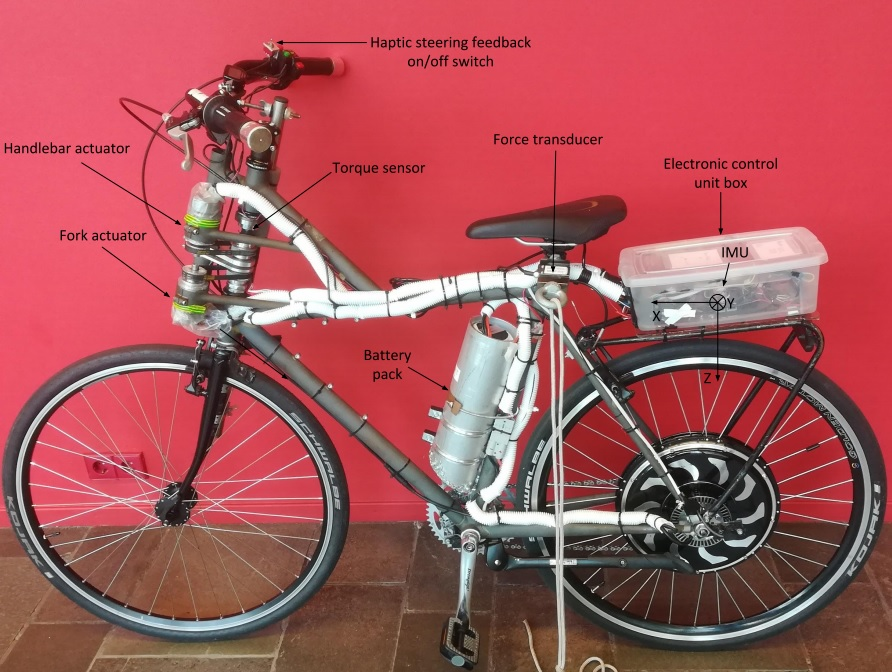
\includegraphics [width=0.8\textwidth]{images/steerbywirebicycle.jpg}
\caption{Prototype of the steer-by-wire bicycle with steering and handlebar actuators, sensors, digital controller and custom made battery pack.}
\label{steerbywireprototype}
\end{figure}

\subsection{Description of steer-by-wire controller} 

To minimize the difference between the handlebar angle $\theta$ and the fork angle $\delta$, tracking control has been implemented. In this way, the steer-by-wire system should behave like an ordinary, mechanically steered bicycle, when the rider applies a steer torque at the handlebar. Two proportional-differential PD-controllers are implemented in order to provide an action-reaction torque $T_{PDH}$ to the handlebar and $T_{PDF}$ to the fork assembly. Angular velocity $\dot{\theta}$ and  $\dot{\delta}$ are estimated by taking the time derivative of angular position $\theta$ and $\delta$ respectively, for a fixed time interval of 1 ms. The double PD-configuration can also be used to manipulate the steer feedback torque independent of the tracking performance. The double PD-controller is of the following form:


\begin{equation}
T_{PDF}=K_{PF}(\theta-\delta)+K_{DF}(\dot{\theta}-\dot{\delta}),
\label{handlebar-controller}
\end{equation}
\begin{equation}
T_{PDH}=K_{PH}(\theta-\delta)+K_{DH}(\dot{\theta}-\dot{\delta})
\label{fork-controller}
\end{equation}

with proportional gains $K_{PH}$, $K_{PF}$ and differential gains $K_{DH}$, $K_{DF}$ respectively. The torque $T_{PDH}$ is applied at the upper servomotor, and the torque $T_{PDF}$ at the lower servomotor. By setting $T_{PDH}$ to zero a steering configuration is created where the rider feels no reaction torque from the steering assembly (feedback "off"), without majorly affecting tracking error performance. The current controller configuration performs with high level of accuracy up to 3 Hz, the tracking error is kept below 3 degrees. However, in certain conditions non-linear effects of the servomotors and tires might create a delay in the control loop effecting the tracking error and realism of the haptic steering feel.


\subsection{Experimental Procedure}

Twenty healthy subjects volunteered in this study. To assure safety all subjects were requested to wear protective equipment in the shape of a standards-approved bike helmet, knee and elbow pads. All participants gave informed consent according to the guidelines of the human research ethics committee of Delft University of Technology. All subjects were healthy and reported that they did not experience any kind of pain or injury in the year before the experiments. The mean weight of all subjects was selected to be close to the European population \cite{walpole2012weight}.

Each experiment trial consisted of four different speeds (i.e., 2.6, 3.7, 4.5, 5.6 \si{\meter\per s}). Two individual trials were performed in total for every speed. In the first trial steering feedback was enabled, whereas in the second trial steering feedback was disabled. Every trial had a duration of approximately 60 seconds. All experiments were performed across Heertjeslaan cycling path of TU Delft, the subjects were requested to ride the steer-by-wire bicycle in all aforementioned speeds while being laterally perturbed. An additional bicycle was used from the experiment coordinator to cycle next to the instrumented steer-by-wire bicycle and perturb the subject, see figure \ref{lateralexperiment}. A set-up which allowed both push and pulls was initially tested but the pushes were subject to inconsistencies. After inspecting the data of the pilot runs, it was observed that unilateral disturbances did not affect the predictability of the perturbation, as the response of the rider was similar. For this reason the unilateral approach was chosen. Nevertheless, to avoid any feedforward control behaviour (e.g., seeing the coordinator preparing to pull the rope) all subjects were asked to keep their focus on the road ahead. 

\begin{figure}[htbp]
\centering
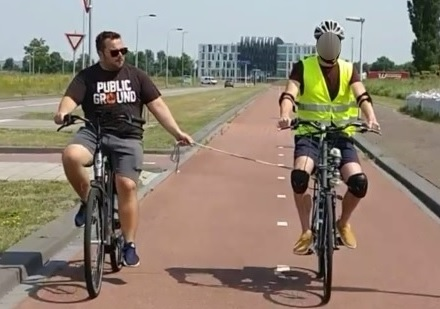
\includegraphics [width=0.8\textwidth]{images/lateralexperiment.jpg}
\caption{Experimental trial performed across Heertjeslaan cycling path of TU Delft; Experiment coordinator cycling next to steer-by-wire bicycle while pulling laterally the subject with a rope.}
\label{lateralexperiment}
\end{figure}

\subsection{System Identification}

In order to remove the effects of unwanted disturbances and noise, the  measured steering angle and estimated  roll angle signals were filtered through a finite impulse response (FIR) model. The impulse response function is defined as the function \(h(\tau)\) which when convoluted with external input \(w(t)\) results in the output \(y(t)\). The output data either represents \(y(t)=\phi(t)\) corresponding to \(h_\phi(\tau)\) or \(y(t)=\delta(t)\) corresponding to \(h_\delta(\tau)\). In discrete time the convolution can be approximated by the following equation:
\begin{equation}
\label{eq:1}
y(t)=\sum_{\tau=0}^{T-1} h(\tau) w(t-\tau)\Delta \tau + v(t)
\end{equation}
where \(T\) is the time length of the impulse function, which  is equal to 3.08 seconds as the oscillations die out after that point and \(v(t)\) the remnant which is caused by unwanted disturbances.
Equation \ref{eq:1} is rewritten in matrix form as follows:
\begin{equation}
\label{eq:2}
y=Wh+v
\end{equation}
where W is the matrix containing time shifted versions of the the input signal.
\begin{equation}
W=\begin{bmatrix} {w(0)} & {0} & {0} & {\dots} & {0} \\ {w(1)} & {w(0)} & {0} & {\dots} & {0} \\ {w(2)} & {w(1)} & {w(0)} & {\dots} & {0} \\ {\vdots} & {\vdots} & {\vdots} & {\ddots} & {0} \\ {w(N-1)} & {w(N-2)} & {w(N-3)} & {\dots} & {w(N-T)}\end{bmatrix}
\end{equation}
Since equation \ref{eq:2} is linear in the parameters (the coefficients of h) there exists a unique solution that can be found through the least squares method.
\begin{equation}
\hat{h}=\left(W^{T} W\right)^{-1} W^{T} y
\end{equation}
Having an estimate of the IRF, the input signal is convoluted with (\(\hat{h}\)) in order to produce  an estimate of the output (\(\hat{y}\))  without the noise. The estimated responses are further smoothed using a eight-order Butterworth filter with cutoff frequency of 10 Hz.


\subsection{Comparison Metrics}
In order to correctly assess if there is a statistically significant difference between the two conditions, three metrics are defined. The first one is the  Power Spectral Centroid (PSC) of measured angle (\(\delta\)) defined as 
\begin{equation}
(PSC_x , PSC_y) =\Bigg( \frac{\sum_{n=1}^{N} f(n) S_\delta(n)}{\sum_{n=1}^{N} S_\delta(n)},\frac{\sum_{n=1}^{N}  S_
\delta(n)^2}{\sum_{n=1}^{N} S_\delta(n)}\Bigg)
\end{equation}

where N is the number of samples lower than 5 Hz and \(S_\delta(f)\) the power spectral density of the signal. This metric gives an indication of the frequency  which most of the power in the signal is centered around. Higher value of \(PSC_x\) will indicate more oscillatory behaviour for the steering response and can be used as a metric of control effort.

The variance accounted for (VAF) is  used to assess  the quality of the fit of the FIR model output. The runs which scored lower than 60\% were removed from further analysis as it was deemed that the model did not sufficiently capture the characteristics of the raw signal. The VAF between  \(\hat{h}_\phi^{off}\) and \(\hat{h}_\phi^{on}\) is also used as a metric of similarity for the roll angle response. In that case VAF is defined as :
\begin{equation}
\mathrm{VAF}_{\phi}=\left(1-\frac{\operatorname{var}\left(\hat{h}_\phi^{off}-\hat{h}_\phi^{on}\right)}{\operatorname{var}\left(\hat{h}_\phi^{off}\right)}\right) \cdot 100 \%
\label{eq:3}
\end{equation}


Finally as a third test, the relative delay between the steering angle IRFs of the two conditions is estimated by finding the lag value of maximum cross-correlation between the signals.

\section{Results}

An independent 2-sample  t-test was conducted to compare if there was significant difference (95 \% confidence interval) in steering effort between conditions for all speed levels, see figure \ref{fig:pscentroid}. For the low speed level ( \(2.6 \;\si{\meter\per s}\)) there was no significant difference in \(PSC_x\) for "feedback on" (M = 0.79, SD = 0.08) and "feedback off" (M = 0.76, SD = 0.10) conditions; t(38)=1.00, p=0.3222. For speed  \(3.7\; \si{\meter\per s}\) there was again no significant difference in the metric for "feedback on" (M = 0.92, SD = 0.11) and "feedback off" (M = 0.92, SD = 0.11); t(38)= -- 1.03, p=0.3075. For  \( 4.5 \;\si{\meter\per s}\) there was also no significant difference in the scores for "feedback on" (M = 0.98, SD = 0.14) and "feedback off" (M = 0.98, SD = 0.14); t(38)= -- 1.04, p=0.3062. And finally, for \( 5.6\; \si{\meter\per s}\) no significant difference was found in the \(PSC_x\) for "feedback on" (M = 1.1, SD = 0.16) and "feedback off" (M = 1.1, SD = 0.16) conditions; t(38)= -- 1.6, p=0.118. 

\begin{figure}[htbp]
\centering
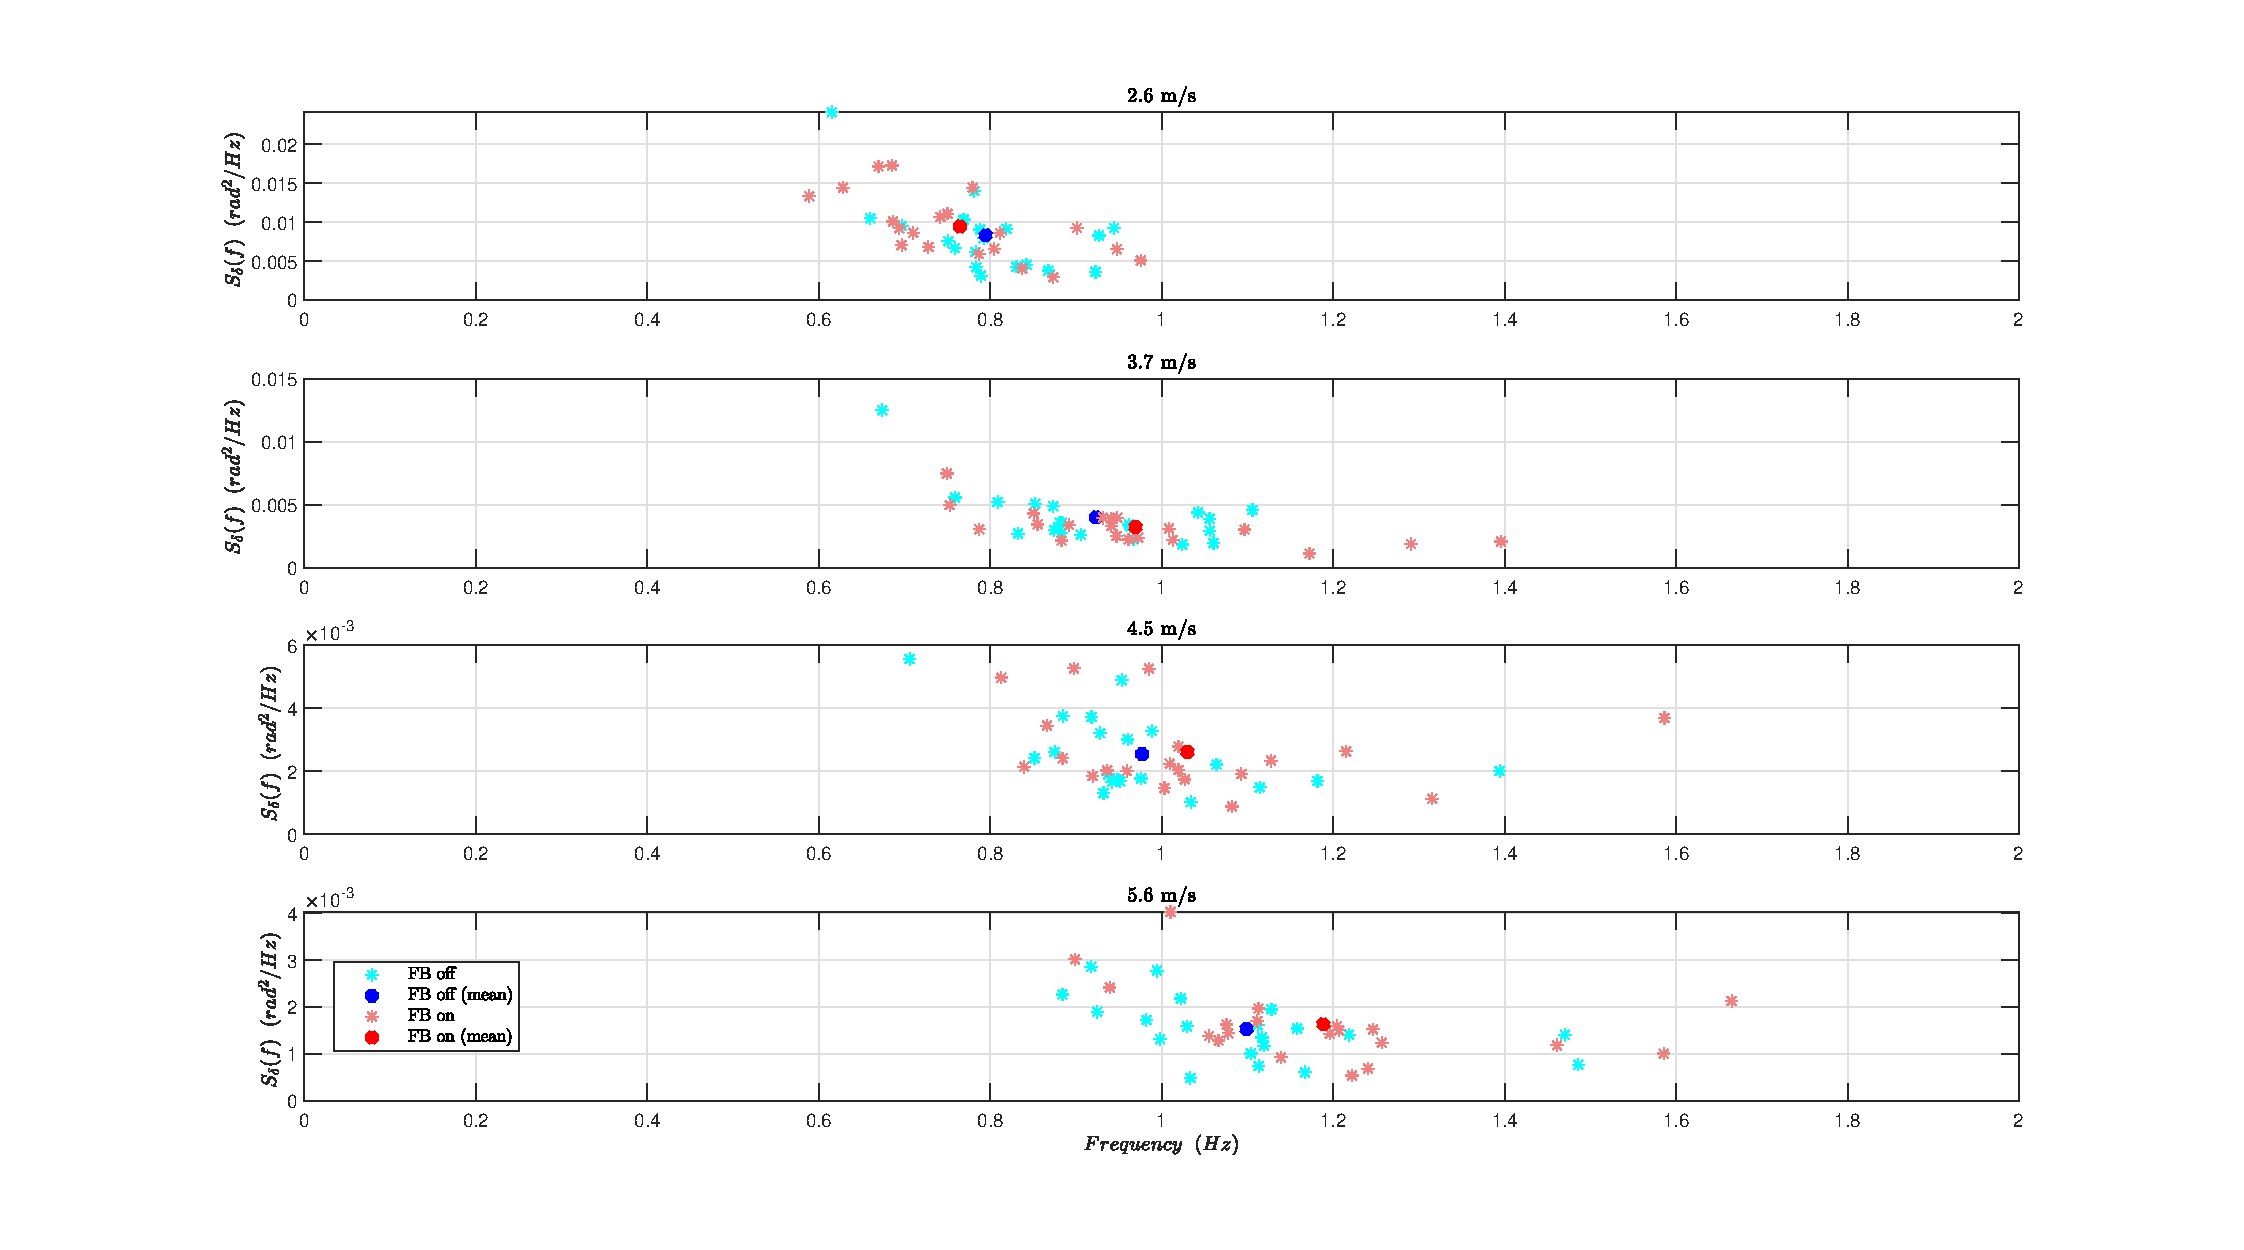
\includegraphics [width=1\textwidth]{images/PSC3.eps}
\caption{The x and y coordinate of the PSC used to determine the frequency where most of the power is concentrated.}
\label{fig:pscentroid}
\end{figure}

The impulse response function of the mean rider for steer angle (\(\delta\)) and roll angle (\(\phi\)) is shown in figure \ref{fig:irf}. The variance accounted for between roll angle impulse responses (see equation \ref{eq:3}) is averaged over all participants and displayed for all speed levels in figure \ref{fig:BoxPlots} (a). Similar roll angle response between "feedback on" and off indicated by higher \(\mathit{VAF}_\phi\) values suggests matching task performance.

\begin{figure}[htbp]
\centering
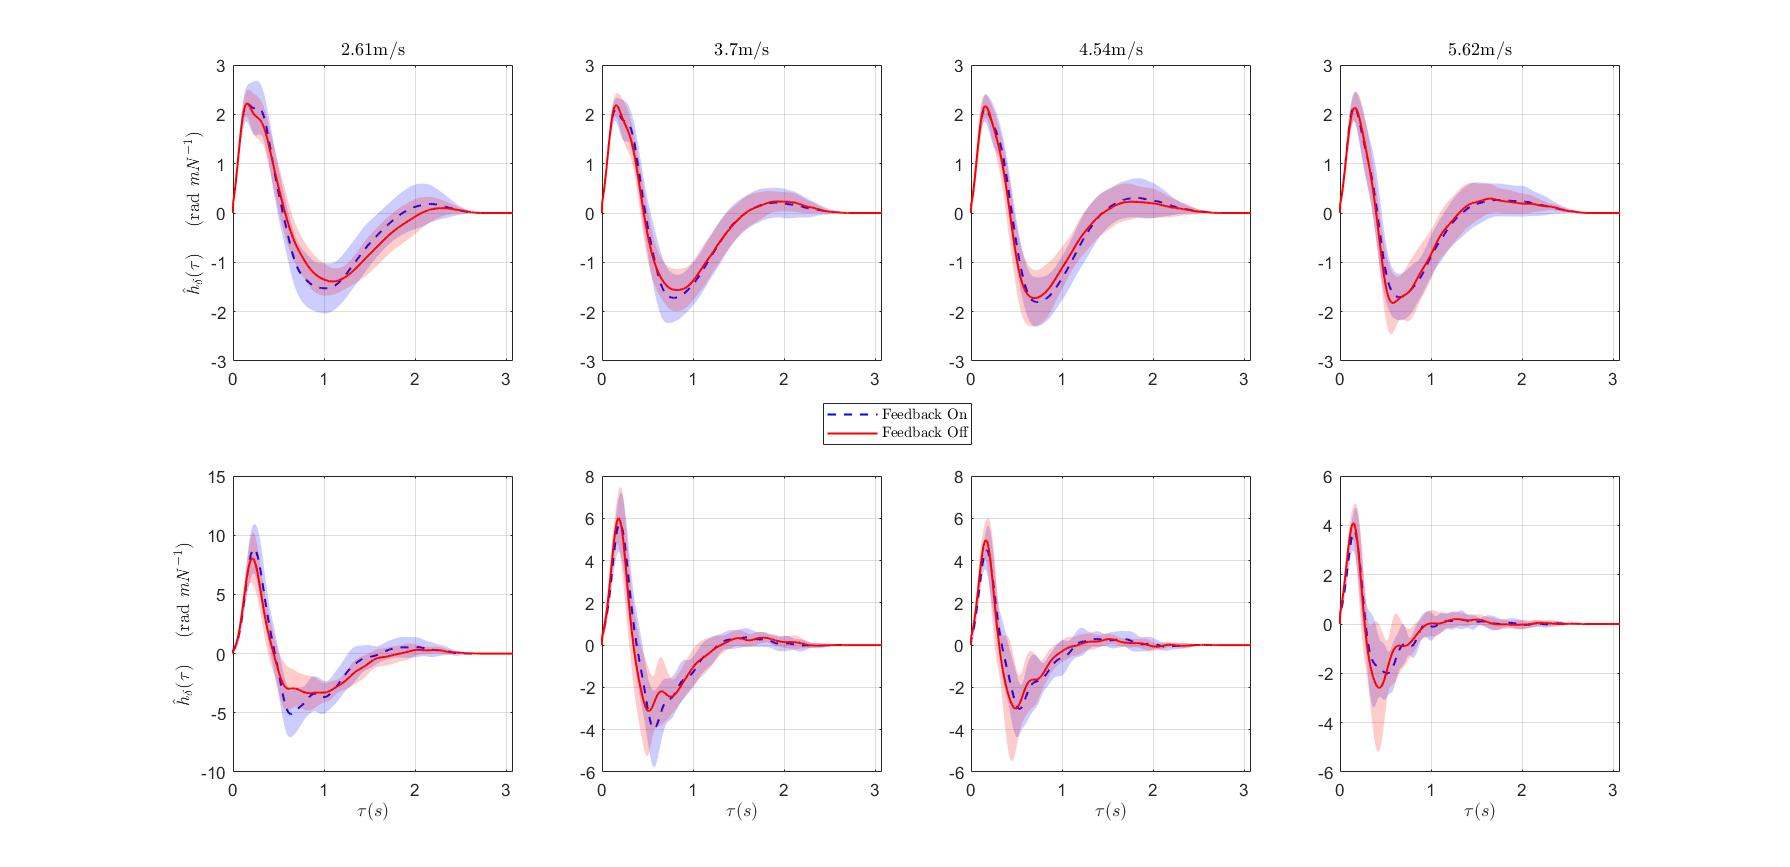
\includegraphics [width=1\textwidth]{images/meanIRF.jpg}
\caption{The impulse response function of the mean rider for steer angle (\(\delta\)) and roll angle (\(\phi\)). The shaded area represents the values within one standard deviation of the mean.}
\label{fig:irf}
\end{figure}

 In addition to the variance roll test an one-sample t-test was conducted to examine if there is any delay in the steering response between feedback on and off, see figure \ref{fig:BoxPlots} (b). For 2.6 m/s there was no significant deviation in the delay (M = -- 3, SD = 25.89) from zero mean; t(19)= -- 0.52, p=0.6103. However, for 3.7 m/s the delay (M = -- 20.65, SD = 25.93) was statistically significant; t(19)= -- 3.56, p=0.0021. Also for 4.5 m/s the mean of the delay (M = -- 23.5, SD = 20.88) was also significantly different than zero; t(19)= -- 5.03, p=0.0001. Lastly, for 5.6 m/s there was again significant difference in the delay (M = -- 19.15, SD = 18.19) from zero; t(19)= -- 4.71, p=0.0002.

% \begin{figure*}[h]
%  \centering
%  \subfigure[]{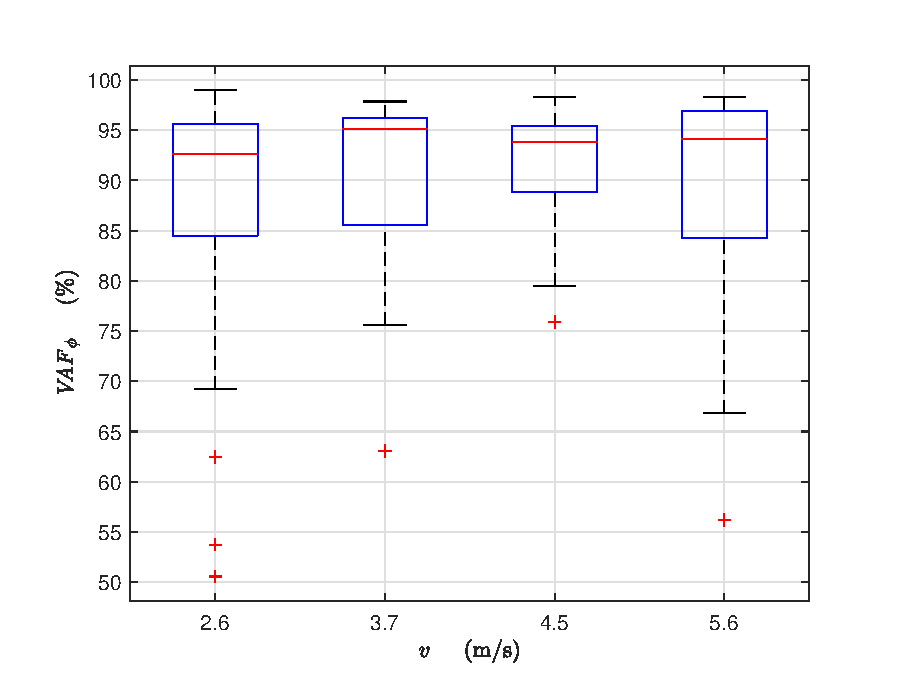
\includegraphics[width=0.61\textwidth]{images/vaf_phi.eps}}
% \subfigure[]{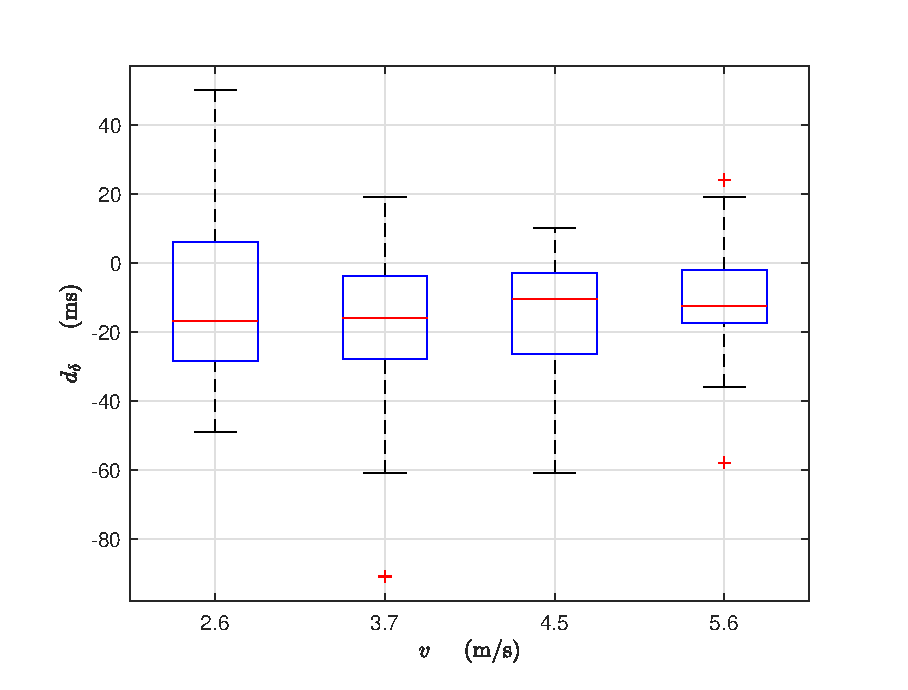
\includegraphics[width=0.61\textwidth]{images/delayBOX.eps}}
%  \caption{ a) Box plot of variance accounted for between roll angle impulse response functions for all speed levels. b) Box plot of the relative delay in the estimated steering angle response  between the two experimental conditions. Negative value means that the "feedback on" signal is delayed compared to the "feedback off".}
% \label{fig:BoxPlots}
% \end{figure*}

% \begin{figure}[h]
%     \centering
%     \begin{subfigure}{0.5\textwidth}
%         \centering
%         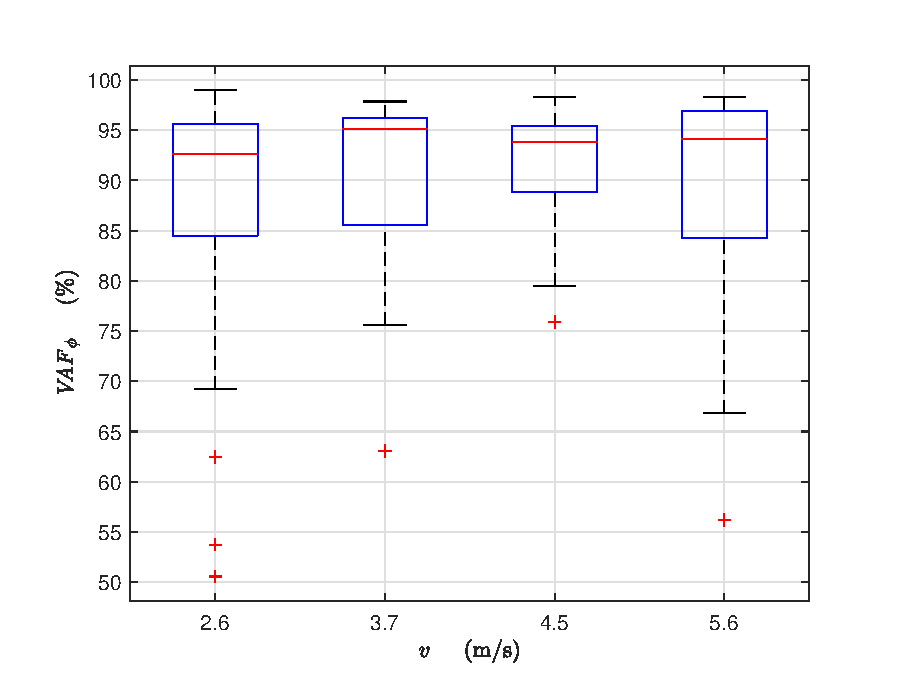
\includegraphics[width=.4\linewidth]{images/vaf_phi.eps}
%         \caption{}
%     \end{subfigure}
%     \begin{subfigure}{0.5\textwidth}
%         \centering
%         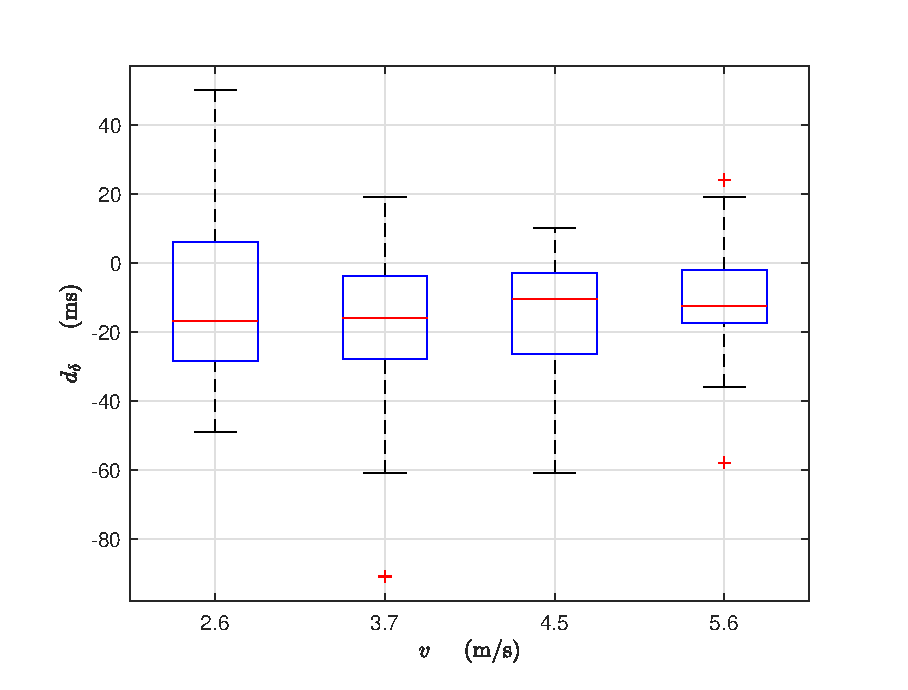
\includegraphics[width=.4\linewidth]{images/delayBOX.eps}
%         \caption{}            
%     \end{subfigure}
%     \caption{ a) Box plot of variance accounted for between roll angle impulse response functions for all speed levels. b) Box plot of the relative delay in the estimated steering angle response  between the two experimental conditions. Negative value means that the "feedback on" signal is delayed compared to the "feedback off".}
%     \label{fig:BoxPlots}
% \end{figure}

\begin{figure}[h]
    \centering{
     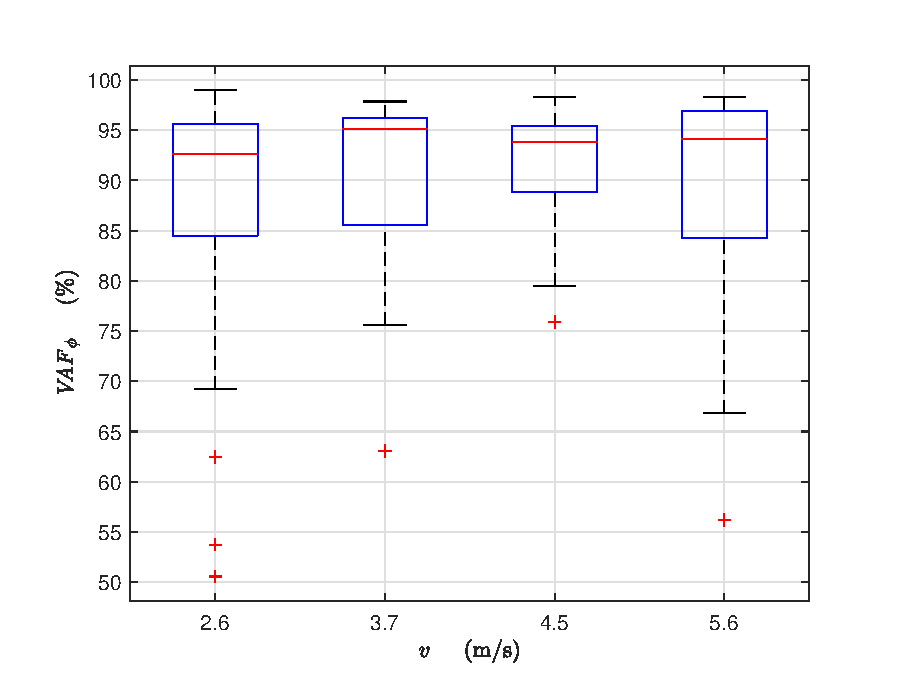
\includegraphics[width=.4\linewidth]{images/vaf_phi.eps}
     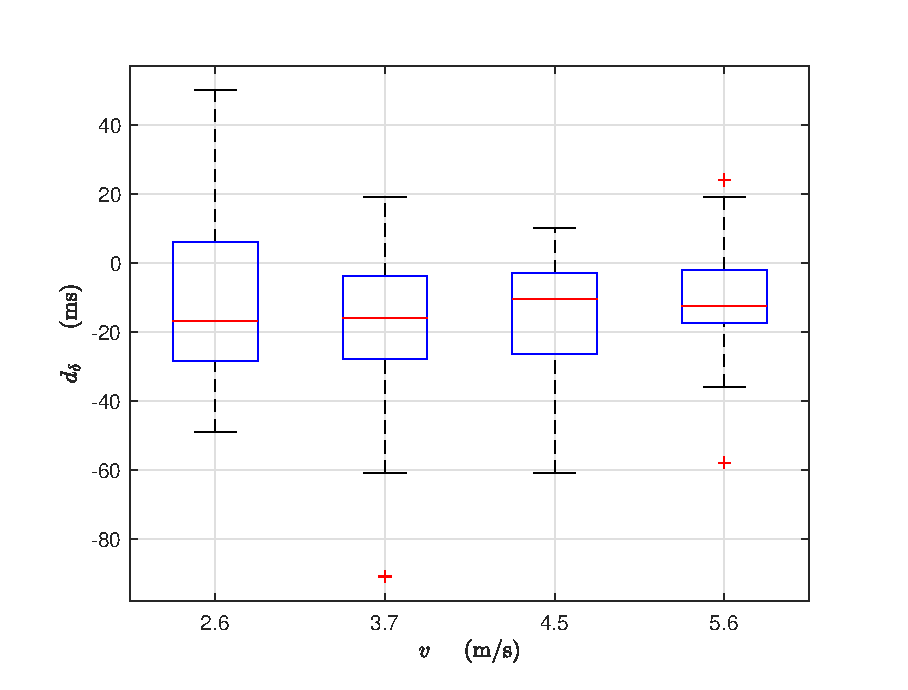
\includegraphics[width=.4\linewidth]{images/delayBOX.eps}

    }
    \caption{ a) Box plot of variance accounted for between roll angle impulse response functions for all speed levels. b) Box plot of the relative delay in the estimated steering angle response  between the two experimental conditions. Negative value means that the "feedback on" signal is delayed compared to the "feedback off".}
    \label{fig:BoxPlots}
\end{figure}

\section{Discussion and Conclusions}

From the aforementioned results it is suggested  that the effects of haptic feedback are minimal to non-existent for the roll stabilization task. Neither performance (see figure \ref{fig:BoxPlots} (a)) or steering effort was affected by the removal of haptic steering feedback. Balance performance among conditions was comparatively consistent  (see figure \ref{fig:BoxPlots} (a)). However, in the unstable speed region the variance and the number of outliers were higher. For steering effort the null hypothesis that the $\mathit{PSC}_x$ metric came from independent random samples with equal means and equal variances failed to be rejected for all speed levels. This does not undoubtedly prove that the samples came from the same population, howbeit it gives a strong indication towards that fact. On the other hand, for the "feedback on"  the steering response was delayed (\(\approx 18\; \si{ms}\) see figure \ref{fig:BoxPlots} (b)) in comparison to the "feedback off". This might be due to the fact that the handlebars are more inert due to the additional steering feedback. 

The lateral pull disturbances can be translated into a lean torque in the direction of forward speed and a steer torque in the direction of the steering axis. This means that any dynamic effects that influences these torques must be examined. The performance of the steer-by-wire controller was examined by numerical simulation and subjective measurements. All subjects reported that they felt like riding a mechanically steered bicycle, no adaptation period was required before the experiments. During the experiments very little motion of the upper body was evident and steer control was expected to be the main mechanism for bicycle balance \cite{moore2011rider}. Thus, we assume that the intristic and reflexives responses of the upperbody do not affect the validity of these results.

Physiologically there are two ways in which proprioception works in order to give the rider information regarding the state of the front assembly. First are the muscle spindles which by detecting changes in velocity and position of the shoulder joint give the rider an estimation of the steering angle and steering rate of the handlebars. Second are the Golgi tendon organs which work as force feedback sensors. The sensory information provided by the latter sensor is what this experiment tried to invalidate. In the feedback on case, information from the ground reaction torque of the front tire is transferred through the handlebars to the sensory receptors of the rider arms and is used for further state estimation. In the feedback off case the steering feedback information is lost. 

Despite the change in the dynamics of the upper handlebar the response of the rider is almost identical. Thereupon, we assume that the internal controller of the rider is either adaptive or is driven by some combination of torque or position control. In the case of torque control this would mean complete re-adaptation of feedback gains which would have resulted in some kind of adaptation period for the  participants when they swapped steering configurations. Although, no adaptation period was needed for any of the participants. Alternatively, in the case of position control steer angle increments are feed-through an inverse model of the steering assembly to produce the necessary forcing element. In this case, switching between configurations, would mean re-adaptation of the internal model of the handlebar assembly. This is much more plausible as it mainly concerns tuning of the internal perception of handlebar inertia which can happen instantaneously. To reveal if the later assumption is true an additional study  that models the rider as position and torque controller will be conducted. The identified parameters of the former and later controller might lead into further insights regarding the conclusions of this study. 

\newpage



\vfill{All data and supplemental material related to this article is available online at \url{https://doi.org/10.5281/zenodo.3365351} (Dialynas et al., 2019)}. 

% \references{report}


  





